% Whitepaper insertion bundle generated from automated studies.
% Usage in ieee_dem_whitepaper.tex:
% % Whitepaper insertion bundle generated from automated studies.
% Usage in ieee_dem_whitepaper.tex:
% % Whitepaper insertion bundle generated from automated studies.
% Usage in ieee_dem_whitepaper.tex:
% % Whitepaper insertion bundle generated from automated studies.
% Usage in ieee_dem_whitepaper.tex:
% \input{whitepaper_bonus_updates.tex}

\subsection{Automated Update Bundle}
The following subsections were generated directly from reproducible scripts and logs.

\input{whitepaper_recent_findings.tex}

\input{part18_findings.tex}

\begin{figure}[!t]
    \centering
    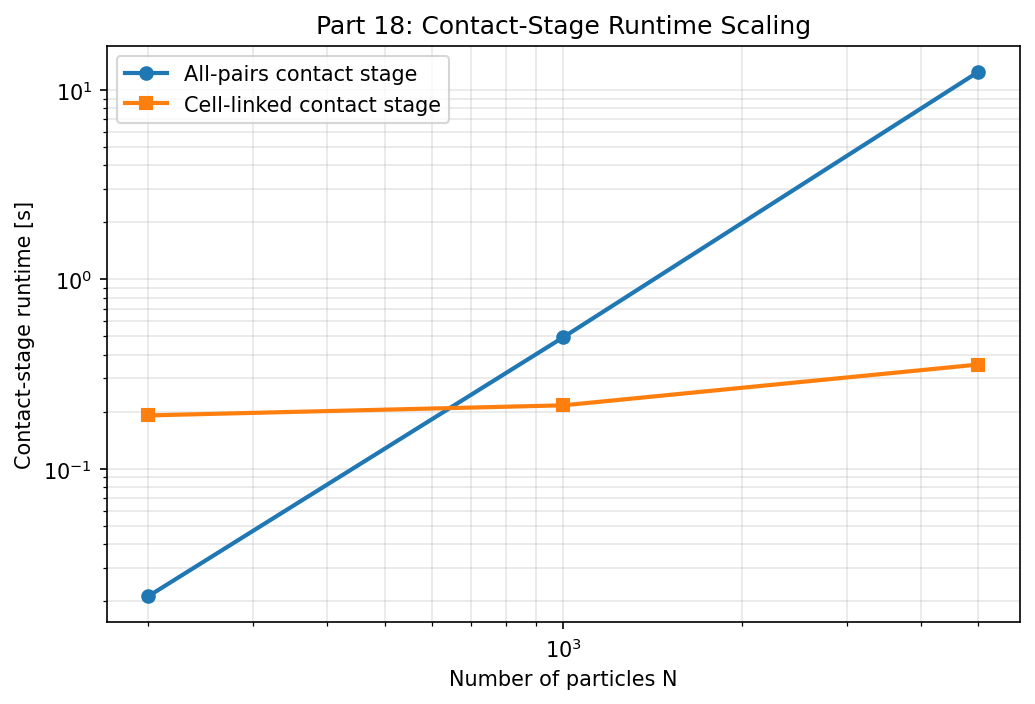
\includegraphics[width=\columnwidth]{part18_contact_runtime.png}
    \caption{Part 18: contact-stage runtime comparison between all-pairs and cell-linked methods.}
    \label{fig:part18-contact-runtime}
\end{figure}

\begin{figure}[!t]
    \centering
    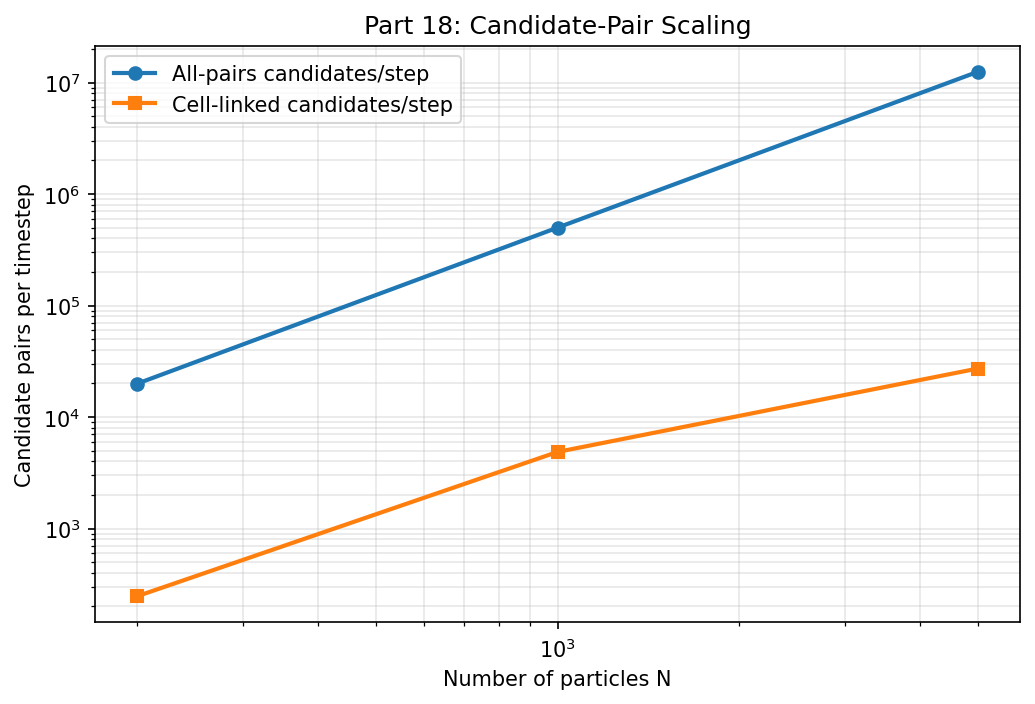
\includegraphics[width=\columnwidth]{part18_candidates.png}
    \caption{Part 18: candidate-pair scaling per timestep for all-pairs and cell-linked search.}
    \label{fig:part18-candidates}
\end{figure}

\input{part19_2_findings.tex}

\begin{figure}[!t]
    \centering
    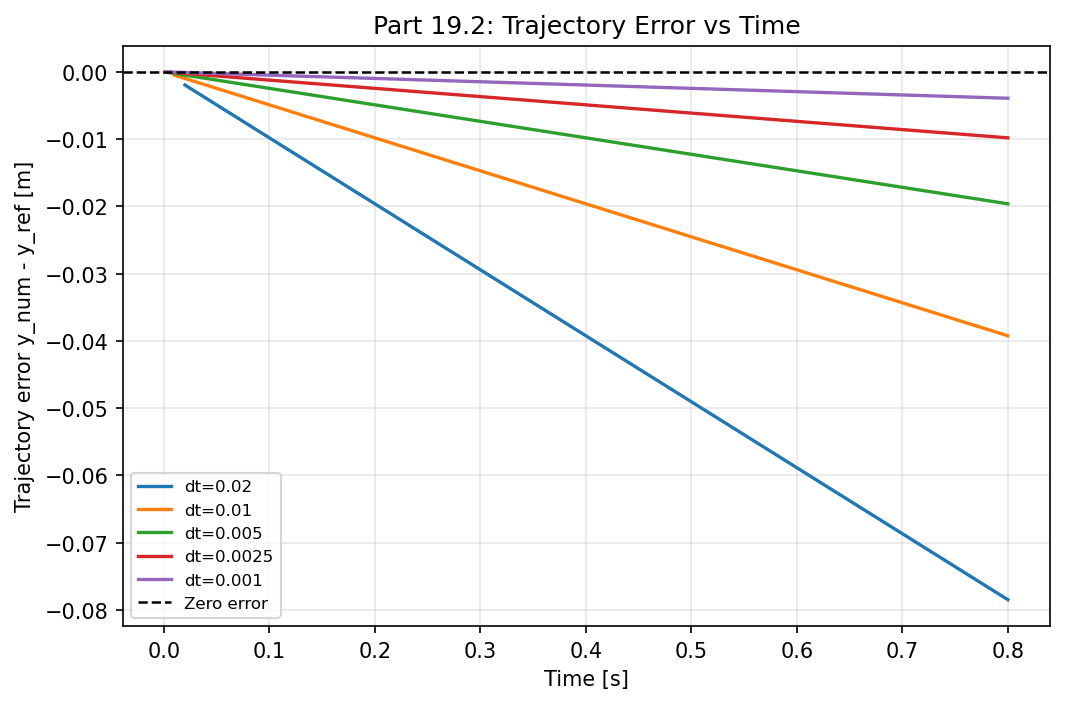
\includegraphics[width=\columnwidth]{part19_2_trajectory_error_overlay.png}
    \caption{Part 19.2: numerical trajectory error against analytical free-fall solution for multiple timesteps.}
    \label{fig:part19-trajectory}
\end{figure}

\begin{figure}[!t]
    \centering
    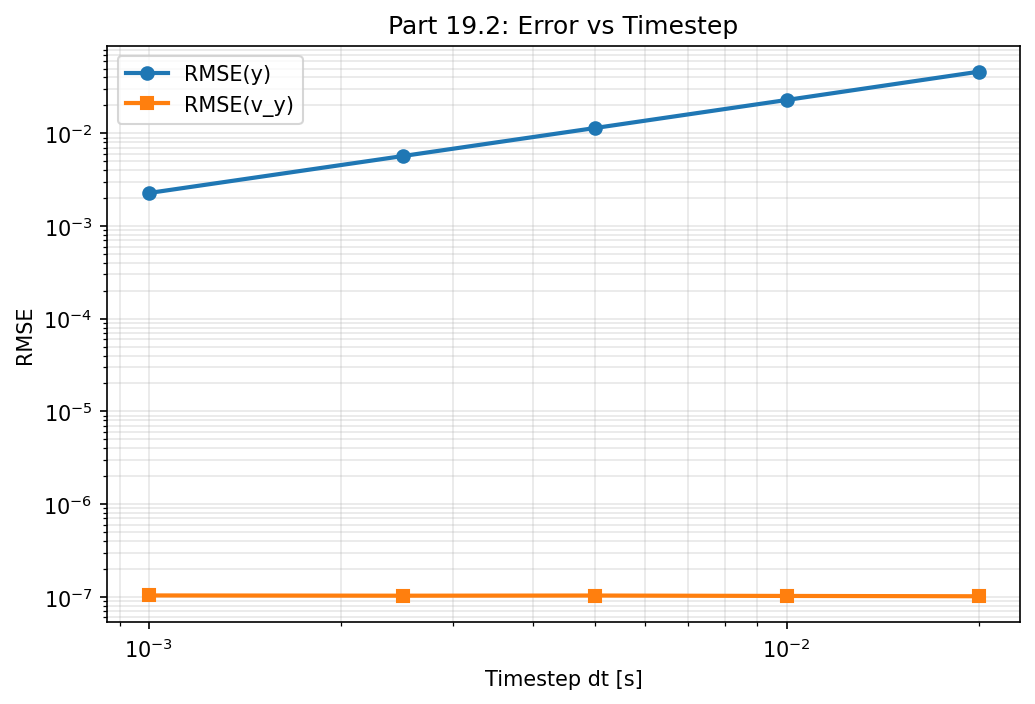
\includegraphics[width=\columnwidth]{part19_2_error_vs_dt.png}
    \caption{Part 19.2: error versus timestep.}
    \label{fig:part19-error-dt}
\end{figure}

\begin{figure}[!t]
    \centering
    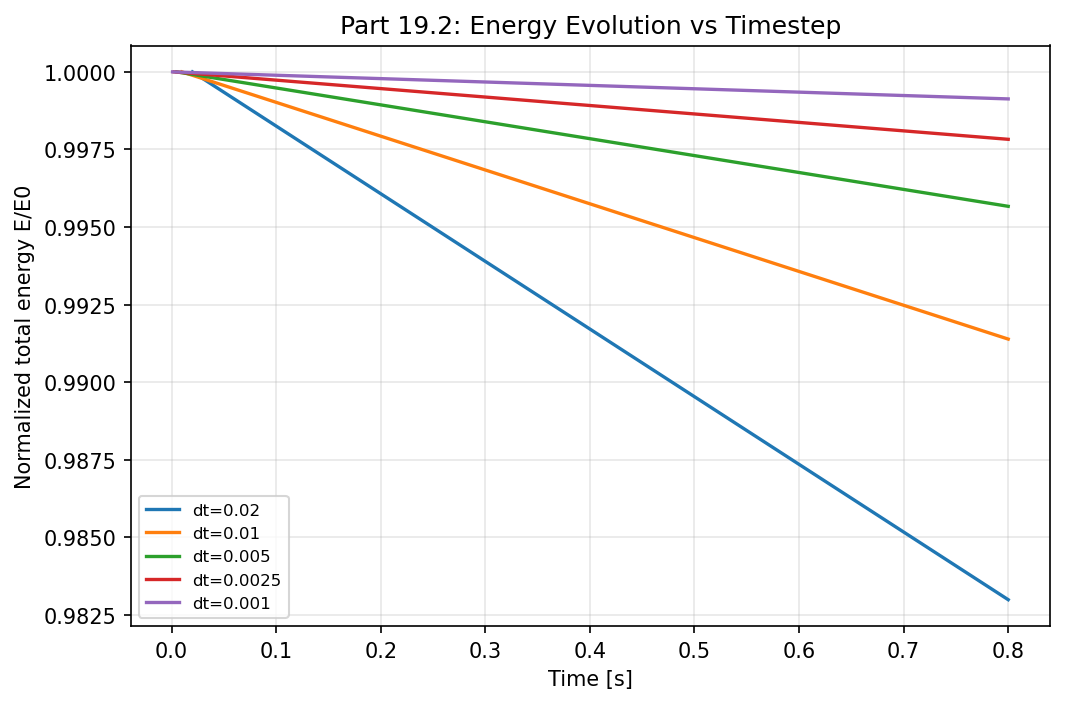
\includegraphics[width=\columnwidth]{part19_2_energy_evolution.png}
    \caption{Part 19.2: normalized total energy evolution for multiple timesteps.}
    \label{fig:part19-energy-evolution}
\end{figure}


\subsection{Automated Update Bundle}
The following subsections were generated directly from reproducible scripts and logs.

\subsection{Implementation and Validation Log (April 2026)}
The following updates were completed and logged for direct inclusion in the white paper.

\subsubsection{Bounce-Detection Robustness in Post-Processing}
The verification workflow was updated in \texttt{test\_verification.py} to avoid false bounce counts when output files were generated from a configuration different from \texttt{input\_config.in}. Two changes were applied:
\begin{enumerate}
    \item Physical time is now read from each VTK header (``Particle data at time ...'') rather than inferred only from a single external configuration file.
    \item Impact detection now uses a ground-contact-aware condition based on particle radius, combined with velocity sign-change and local-minimum filtering, followed by a small temporal de-duplication window.
\end{enumerate}
With these changes, the tuned bounce case reports five impacts in the $8\,\mathrm{s}$ analysis window at approximately $t=[0.96,\,2.79,\,4.54,\,6.22,\,7.82]$ s.

\subsubsection{Serial Profiling (Part 12)}
A dedicated profiling run was logged in \texttt{part12\_serial\_profile.csv} and \texttt{part12\_profile\_report.txt}. For case \texttt{part10\_n5000}, the measured serial runtime and distribution were:
\begin{itemize}
    \item total runtime: $2.0731\,\mathrm{s}$
    \item particle contact stage: $2.0384\,\mathrm{s}$ ($98.33\%$)
    \item output stage: $3.0803\times10^{-2}\,\mathrm{s}$ ($1.49\%$)
\end{itemize}
The dominant computational bottleneck is therefore the particle--particle contact stage.

\subsubsection{Parallel Correctness Checks (Part 13)}
Serial-vs-OpenMP comparisons were logged in \texttt{parallel\_validation\_report.csv} for $N=200,1000,5000$ and thread counts $p=2,4,8$. All checks returned \texttt{PASS} with
\begin{itemize}
    \item max absolute position difference: $0.0$
    \item max absolute velocity difference: $0.0$
    \item max absolute kinetic-energy difference: $0.0$
\end{itemize}
under the configured tolerances.

\subsubsection{Scaling and Amdahl Interpretation (Part 14)}
Performance artifacts were generated through \texttt{performance\_raw.csv}, \texttt{performance\_speedup.csv}, and \texttt{performance\_amdahl\_fit.csv}. Selected results at $p=8$ are:
\begin{itemize}
    \item $N=200$: $S(8)=0.969$, $E(8)=0.121$
    \item $N=1000$: $S(8)=1.722$, $E(8)=0.215$
    \item $N=5000$: $S(8)=2.248$, $E(8)=0.281$
\end{itemize}
This trend indicates that small systems are overhead-dominated, while larger systems amortize OpenMP overhead better. Fitted Amdahl serial fractions were approximately $f\approx0.49$ ($N=1000$) and $f\approx0.47$ ($N=5000$), consistent with non-ideal scaling.


\subsection{Bonus Part 18: Neighbour-Search Comparison}
A switchable contact-search implementation was added with \texttt{contact\_search\_method=0} (all-pairs) and \texttt{contact\_search\_method=1} (cell-linked).
Empirical candidate-pair scaling from the measured data is approximately $\mathcal{O}(N^{2.00})$ for all-pairs and $\mathcal{O}(N^{1.46})$ for the cell-linked strategy.
\begin{table}[!t]
\scriptsize
\centering
\caption{Part 18 neighbour-search comparison (serial runs)}
\label{tab:part18-neighbour-search}
\begin{tabular}{rcccccccc}
\toprule
$N$ & $t_{tot}^{AP}$ & $t_{tot}^{CL}$ & $S_{tot}$ & $t_c^{AP}$ & $t_c^{CL}$ & $S_c$ & Cand. factor \\
\midrule
200 & 0.0226 & 0.1932 & 0.12 & 0.0212 & 0.1914 & 0.11 & 80.57 \\
1000 & 0.5019 & 0.2230 & 2.25 & 0.4955 & 0.2164 & 2.29 & 102.69 \\
5000 & 12.5362 & 0.3839 & 32.66 & 12.5061 & 0.3554 & 35.18 & 458.85 \\
\bottomrule
\end{tabular}
\end{table}
where $t_{tot}^{AP}, t_{tot}^{CL}$ are total runtimes; $t_c^{AP}, t_c^{CL}$ are contact-stage runtimes; $S_{tot}, S_c$ are the corresponding cell-linked speedups over all-pairs; and Cand. factor is the candidate-pair ratio $N_{cand}^{AP}/N_{cand}^{CL}$.
Detected-contact counts match between methods for each tested $N$, confirming contact-search correctness while reducing candidate checks.
The measured candidate-pair reduction confirms why the baseline all-pairs method behaves as the expensive $\mathcal{O}(N^2)$ reference algorithm.
For small systems (here $N=200$), the cell-linked method is slower than all-pairs because grid build and traversal overheads dominate the reduced pair-check count.


\begin{figure}[!t]
    \centering
    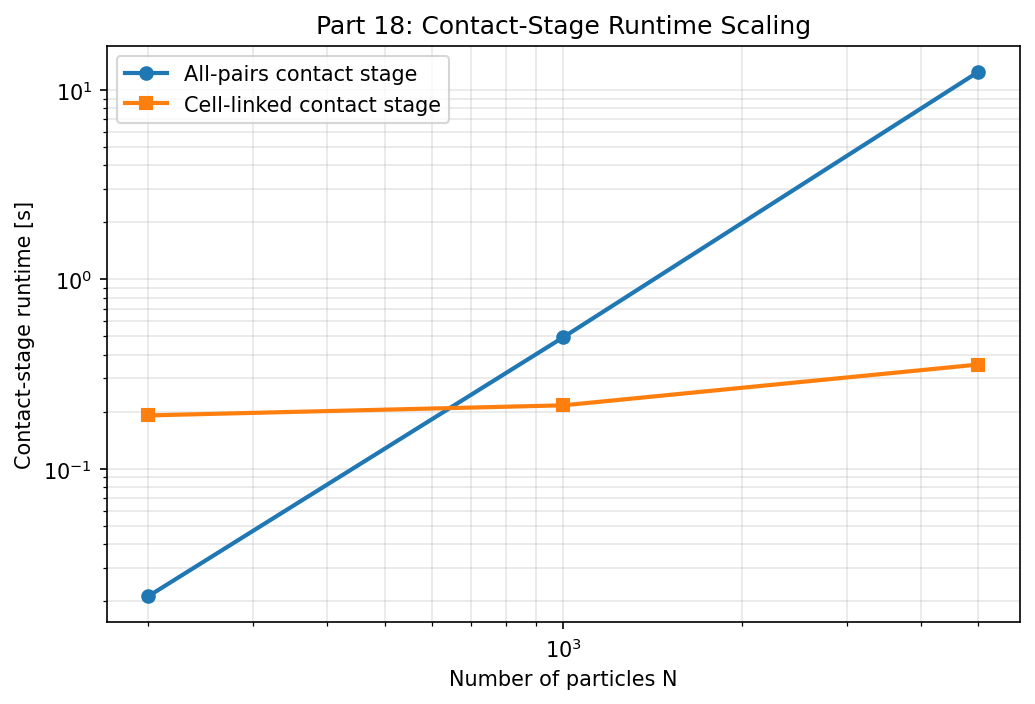
\includegraphics[width=\columnwidth]{part18_contact_runtime.png}
    \caption{Part 18: contact-stage runtime comparison between all-pairs and cell-linked methods.}
    \label{fig:part18-contact-runtime}
\end{figure}

\begin{figure}[!t]
    \centering
    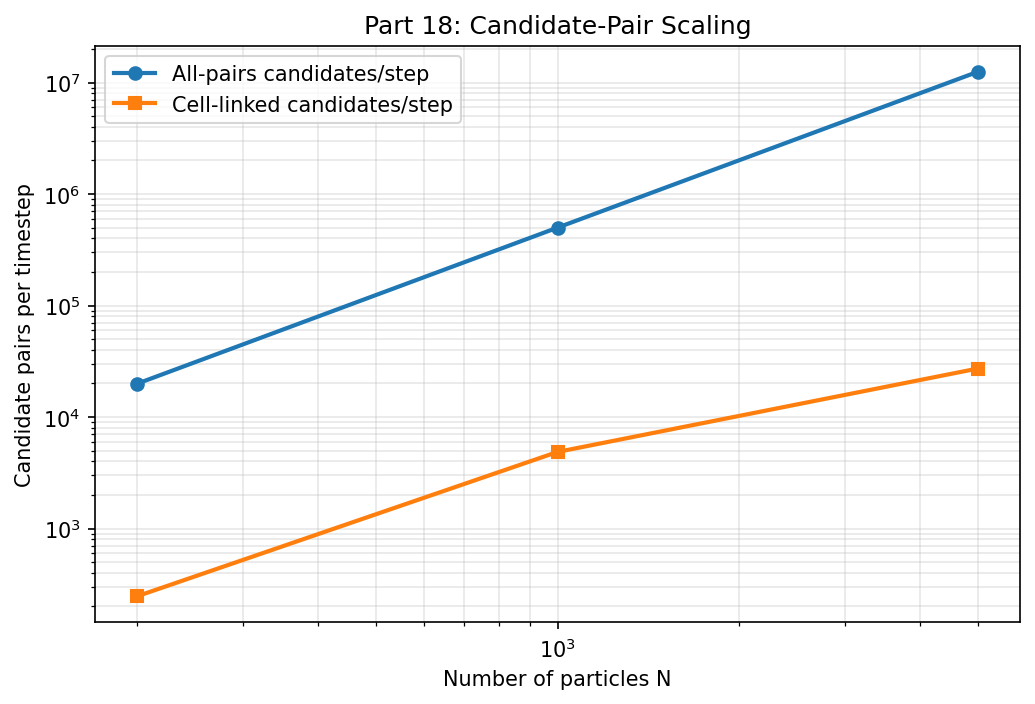
\includegraphics[width=\columnwidth]{part18_candidates.png}
    \caption{Part 18: candidate-pair scaling per timestep for all-pairs and cell-linked search.}
    \label{fig:part18-candidates}
\end{figure}

\subsection{Bonus Part 19.2: Timestep Sensitivity and Stability Limit}
A free-fall case without wall contact was simulated for multiple timesteps to quantify numerical accuracy and energy behavior.
\begin{table}[!t]
\centering
\caption{Part 19.2 timestep sensitivity metrics}
\label{tab:part19-2-timestep}
\begin{tabular}{rcccc}
\toprule
$\Delta t$ [s] & RMSE$(y)$ [m] & RMSE$(v_y)$ [m/s] & Max $|\Delta y|$ [m] & Max energy drift \\
\midrule
0.0200 & 4.616e-02 & 1.013e-07 & 7.848e-02 & 1.701e-02 \\
0.0100 & 2.287e-02 & 1.021e-07 & 3.924e-02 & 8.612e-03 \\
0.0050 & 1.138e-02 & 1.031e-07 & 1.962e-02 & 4.333e-03 \\
0.0025 & 5.677e-03 & 1.027e-07 & 9.810e-03 & 2.173e-03 \\
0.0010 & 2.268e-03 & 1.034e-07 & 3.924e-03 & 8.708e-04 \\
\bottomrule
\end{tabular}
\end{table}
A log-log fit gives an error slope of approximately 1.01 for position RMSE, which is consistent with first-order temporal behavior expected from semi-implicit Euler integration.
Velocity RMSE remains nearly timestep-independent at about 1e-7 m/s across all tested timesteps (slope -0.01), indicating that truncation error in this observable is already below a small floating-point and interpolation floor for this setup.
A Richardson three-grid analysis on final-height values gives observed orders between 1.00 and 1.00 (mean 1.00), consistent with first-order time integration.
\begin{table}[!t]
\centering
\caption{Part 19.2 Richardson observed order (final height)}
\label{tab:part19-2-richardson}
\begin{tabular}{rcc}
\toprule
$(\Delta t_c,\Delta t_m,\Delta t_f)$ [s] & $r$ & $p_{obs}$ \\
\midrule
(0.0200, 0.0100, 0.0050) & 2.0 & 1.00 \\
(0.0100, 0.0050, 0.0025) & 2.0 & 1.00 \\
\bottomrule
\end{tabular}
\end{table}
To connect this convergence study with stability limits, a bouncing test was run around a theoretical explicit-step threshold. Using a linear spring-mass estimate, the contact time is $t_c \approx \pi\sqrt{m/k_n}$ and the threshold used here is $\Delta t_{crit}=t_c/\pi$ \cite{edem_linear_spring,pfc_timestep}.
For $m=1.3$ kg and $k_n=1.0e+05$ N/m, this gives $t_c\approx 0.0113$ s and $\Delta t_{crit}\approx 0.0036$ s.
\begin{table}[!t]
\centering
\caption{Part 19.2 critical timestep check (bouncing case)}
\label{tab:part19-2-critical}
\begin{tabular}{rccc}
\toprule
$\Delta t$ [s] & $\Delta t/\Delta t_{crit}$ & Max $E/E0$ & Final $E/E0$ \\
\midrule
0.0030 & 0.83 & 1.39 & 0.83 \\
0.0040 & 1.11 & 9.40 & 5.26 \\
\bottomrule
\end{tabular}
\end{table}
The under-limit run ($\Delta t=0.003$ s) remains bounded but shows numerical energy gain (Max $E/E0=1.39$), whereas the over-limit run ($\Delta t=0.004$ s) exhibits rapid unphysical energy growth (Max $E/E0=9.40$), which is visible as a sharp upward trend in the critical-energy plot.


\begin{figure}[!t]
    \centering
    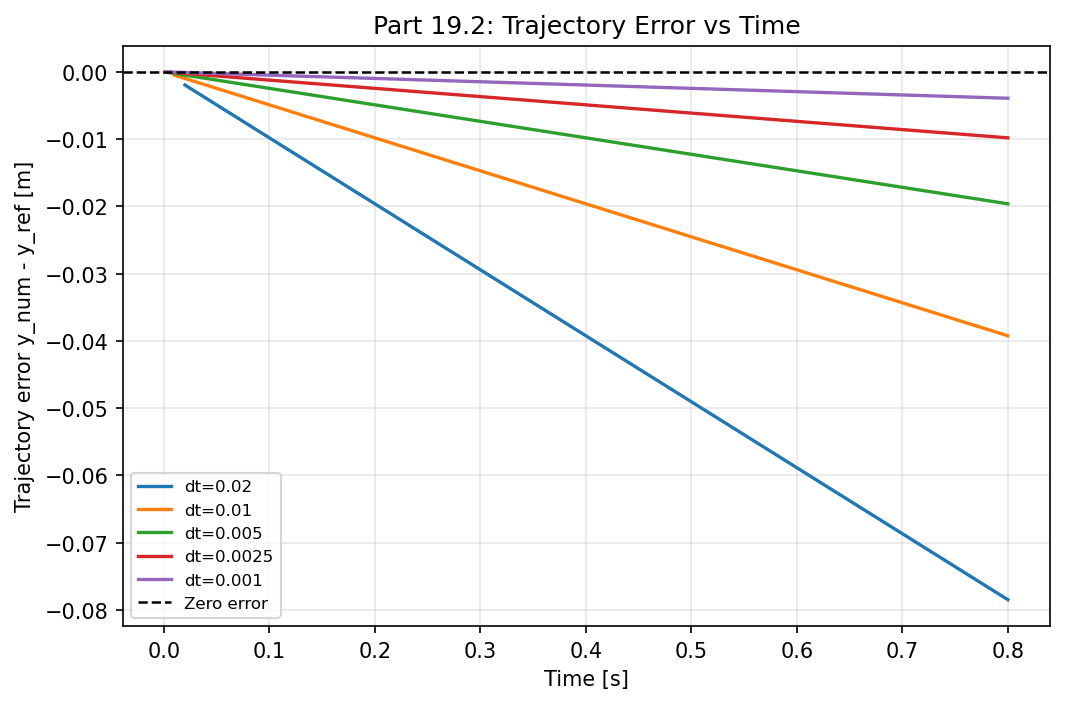
\includegraphics[width=\columnwidth]{part19_2_trajectory_error_overlay.png}
    \caption{Part 19.2: numerical trajectory error against analytical free-fall solution for multiple timesteps.}
    \label{fig:part19-trajectory}
\end{figure}

\begin{figure}[!t]
    \centering
    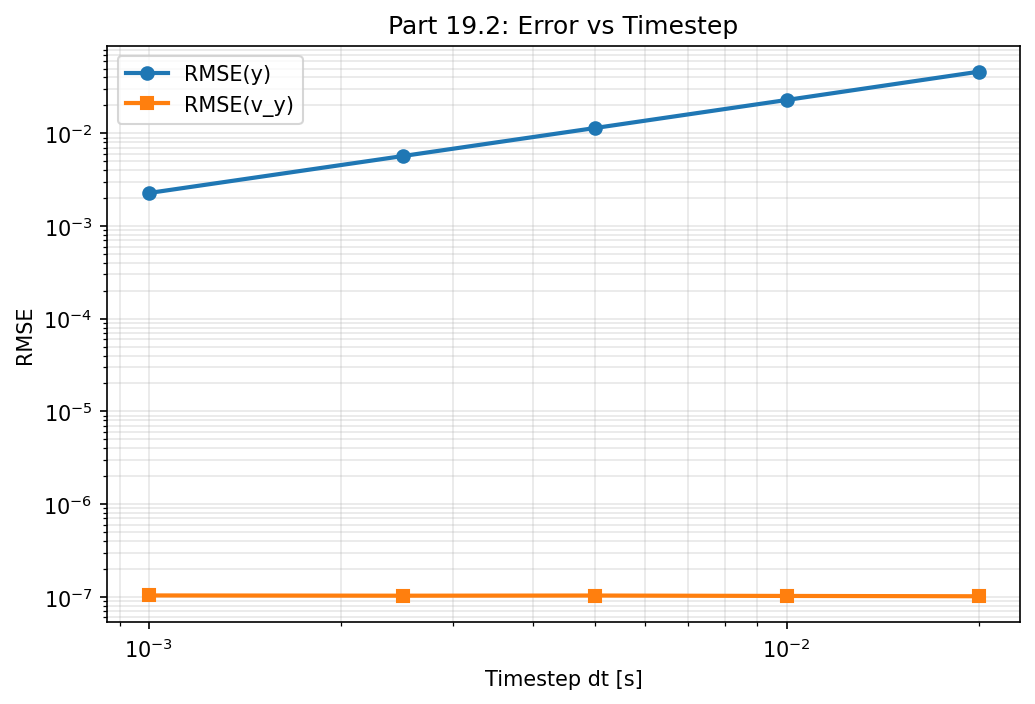
\includegraphics[width=\columnwidth]{part19_2_error_vs_dt.png}
    \caption{Part 19.2: error versus timestep.}
    \label{fig:part19-error-dt}
\end{figure}

\begin{figure}[!t]
    \centering
    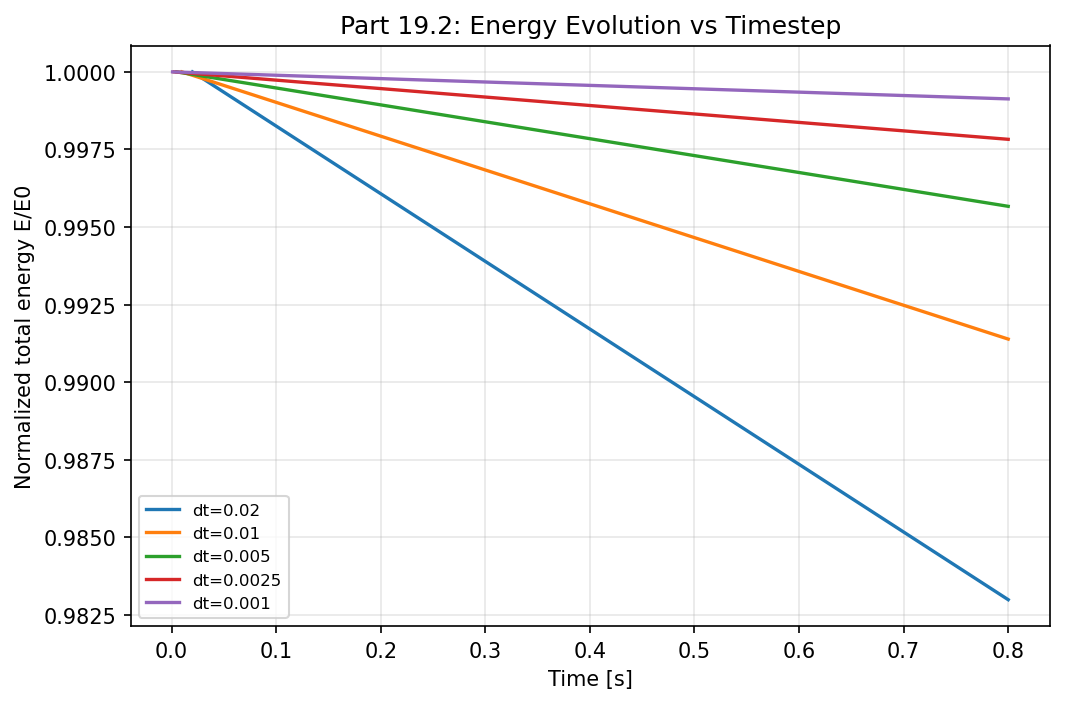
\includegraphics[width=\columnwidth]{part19_2_energy_evolution.png}
    \caption{Part 19.2: normalized total energy evolution for multiple timesteps.}
    \label{fig:part19-energy-evolution}
\end{figure}


\subsection{Automated Update Bundle}
The following subsections were generated directly from reproducible scripts and logs.

\subsection{Implementation and Validation Log (April 2026)}
The following updates were completed and logged for direct inclusion in the white paper.

\subsubsection{Bounce-Detection Robustness in Post-Processing}
The verification workflow was updated in \texttt{test\_verification.py} to avoid false bounce counts when output files were generated from a configuration different from \texttt{input\_config.in}. Two changes were applied:
\begin{enumerate}
    \item Physical time is now read from each VTK header (``Particle data at time ...'') rather than inferred only from a single external configuration file.
    \item Impact detection now uses a ground-contact-aware condition based on particle radius, combined with velocity sign-change and local-minimum filtering, followed by a small temporal de-duplication window.
\end{enumerate}
With these changes, the tuned bounce case reports five impacts in the $8\,\mathrm{s}$ analysis window at approximately $t=[0.96,\,2.79,\,4.54,\,6.22,\,7.82]$ s.

\subsubsection{Serial Profiling (Part 12)}
A dedicated profiling run was logged in \texttt{part12\_serial\_profile.csv} and \texttt{part12\_profile\_report.txt}. For case \texttt{part10\_n5000}, the measured serial runtime and distribution were:
\begin{itemize}
    \item total runtime: $2.0731\,\mathrm{s}$
    \item particle contact stage: $2.0384\,\mathrm{s}$ ($98.33\%$)
    \item output stage: $3.0803\times10^{-2}\,\mathrm{s}$ ($1.49\%$)
\end{itemize}
The dominant computational bottleneck is therefore the particle--particle contact stage.

\subsubsection{Parallel Correctness Checks (Part 13)}
Serial-vs-OpenMP comparisons were logged in \texttt{parallel\_validation\_report.csv} for $N=200,1000,5000$ and thread counts $p=2,4,8$. All checks returned \texttt{PASS} with
\begin{itemize}
    \item max absolute position difference: $0.0$
    \item max absolute velocity difference: $0.0$
    \item max absolute kinetic-energy difference: $0.0$
\end{itemize}
under the configured tolerances.

\subsubsection{Scaling and Amdahl Interpretation (Part 14)}
Performance artifacts were generated through \texttt{performance\_raw.csv}, \texttt{performance\_speedup.csv}, and \texttt{performance\_amdahl\_fit.csv}. Selected results at $p=8$ are:
\begin{itemize}
    \item $N=200$: $S(8)=0.969$, $E(8)=0.121$
    \item $N=1000$: $S(8)=1.722$, $E(8)=0.215$
    \item $N=5000$: $S(8)=2.248$, $E(8)=0.281$
\end{itemize}
This trend indicates that small systems are overhead-dominated, while larger systems amortize OpenMP overhead better. Fitted Amdahl serial fractions were approximately $f\approx0.49$ ($N=1000$) and $f\approx0.47$ ($N=5000$), consistent with non-ideal scaling.


\subsection{Bonus Part 18: Neighbour-Search Comparison}
A switchable contact-search implementation was added with \texttt{contact\_search\_method=0} (all-pairs) and \texttt{contact\_search\_method=1} (cell-linked).
Empirical candidate-pair scaling from the measured data is approximately $\mathcal{O}(N^{2.00})$ for all-pairs and $\mathcal{O}(N^{1.46})$ for the cell-linked strategy.
\begin{table}[!t]
\scriptsize
\centering
\caption{Part 18 neighbour-search comparison (serial runs)}
\label{tab:part18-neighbour-search}
\begin{tabular}{rcccccccc}
\toprule
$N$ & $t_{tot}^{AP}$ & $t_{tot}^{CL}$ & $S_{tot}$ & $t_c^{AP}$ & $t_c^{CL}$ & $S_c$ & Cand. factor \\
\midrule
200 & 0.0226 & 0.1932 & 0.12 & 0.0212 & 0.1914 & 0.11 & 80.57 \\
1000 & 0.5019 & 0.2230 & 2.25 & 0.4955 & 0.2164 & 2.29 & 102.69 \\
5000 & 12.5362 & 0.3839 & 32.66 & 12.5061 & 0.3554 & 35.18 & 458.85 \\
\bottomrule
\end{tabular}
\end{table}
where $t_{tot}^{AP}, t_{tot}^{CL}$ are total runtimes; $t_c^{AP}, t_c^{CL}$ are contact-stage runtimes; $S_{tot}, S_c$ are the corresponding cell-linked speedups over all-pairs; and Cand. factor is the candidate-pair ratio $N_{cand}^{AP}/N_{cand}^{CL}$.
Detected-contact counts match between methods for each tested $N$, confirming contact-search correctness while reducing candidate checks.
The measured candidate-pair reduction confirms why the baseline all-pairs method behaves as the expensive $\mathcal{O}(N^2)$ reference algorithm.
For small systems (here $N=200$), the cell-linked method is slower than all-pairs because grid build and traversal overheads dominate the reduced pair-check count.


\begin{figure}[!t]
    \centering
    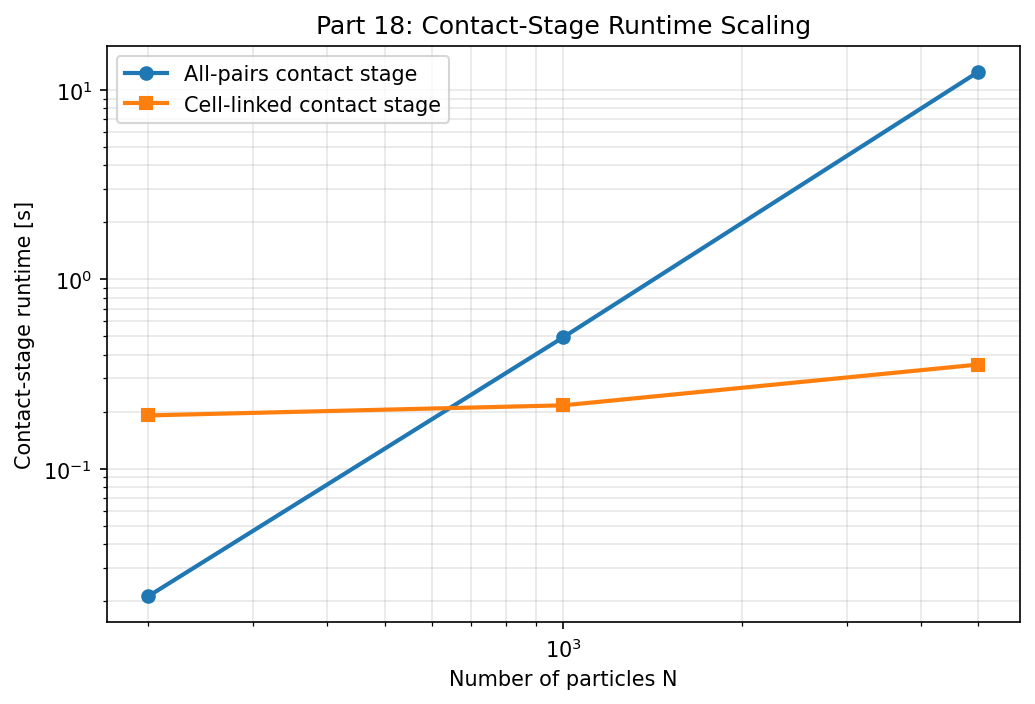
\includegraphics[width=\columnwidth]{part18_contact_runtime.png}
    \caption{Part 18: contact-stage runtime comparison between all-pairs and cell-linked methods.}
    \label{fig:part18-contact-runtime}
\end{figure}

\begin{figure}[!t]
    \centering
    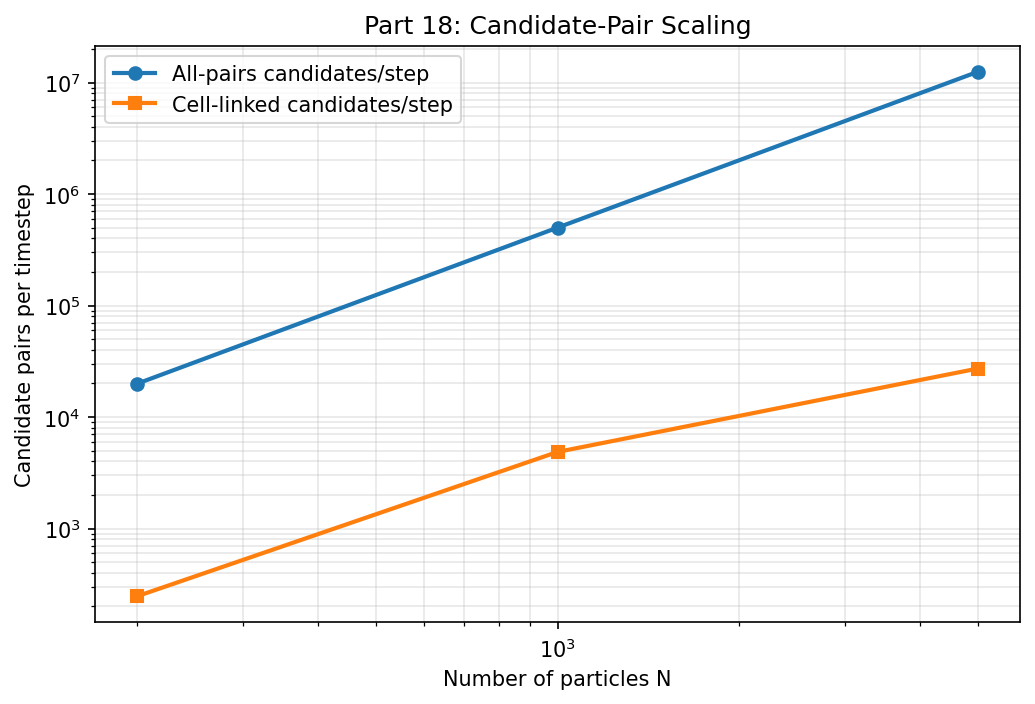
\includegraphics[width=\columnwidth]{part18_candidates.png}
    \caption{Part 18: candidate-pair scaling per timestep for all-pairs and cell-linked search.}
    \label{fig:part18-candidates}
\end{figure}

\subsection{Bonus Part 19.2: Timestep Sensitivity and Stability Limit}
A free-fall case without wall contact was simulated for multiple timesteps to quantify numerical accuracy and energy behavior.
\begin{table}[!t]
\centering
\caption{Part 19.2 timestep sensitivity metrics}
\label{tab:part19-2-timestep}
\begin{tabular}{rcccc}
\toprule
$\Delta t$ [s] & RMSE$(y)$ [m] & RMSE$(v_y)$ [m/s] & Max $|\Delta y|$ [m] & Max energy drift \\
\midrule
0.0200 & 4.616e-02 & 1.013e-07 & 7.848e-02 & 1.701e-02 \\
0.0100 & 2.287e-02 & 1.021e-07 & 3.924e-02 & 8.612e-03 \\
0.0050 & 1.138e-02 & 1.031e-07 & 1.962e-02 & 4.333e-03 \\
0.0025 & 5.677e-03 & 1.027e-07 & 9.810e-03 & 2.173e-03 \\
0.0010 & 2.268e-03 & 1.034e-07 & 3.924e-03 & 8.708e-04 \\
\bottomrule
\end{tabular}
\end{table}
A log-log fit gives an error slope of approximately 1.01 for position RMSE, which is consistent with first-order temporal behavior expected from semi-implicit Euler integration.
Velocity RMSE remains nearly timestep-independent at about 1e-7 m/s across all tested timesteps (slope -0.01), indicating that truncation error in this observable is already below a small floating-point and interpolation floor for this setup.
A Richardson three-grid analysis on final-height values gives observed orders between 1.00 and 1.00 (mean 1.00), consistent with first-order time integration.
\begin{table}[!t]
\centering
\caption{Part 19.2 Richardson observed order (final height)}
\label{tab:part19-2-richardson}
\begin{tabular}{rcc}
\toprule
$(\Delta t_c,\Delta t_m,\Delta t_f)$ [s] & $r$ & $p_{obs}$ \\
\midrule
(0.0200, 0.0100, 0.0050) & 2.0 & 1.00 \\
(0.0100, 0.0050, 0.0025) & 2.0 & 1.00 \\
\bottomrule
\end{tabular}
\end{table}
To connect this convergence study with stability limits, a bouncing test was run around a theoretical explicit-step threshold. Using a linear spring-mass estimate, the contact time is $t_c \approx \pi\sqrt{m/k_n}$ and the threshold used here is $\Delta t_{crit}=t_c/\pi$ \cite{edem_linear_spring,pfc_timestep}.
For $m=1.3$ kg and $k_n=1.0e+05$ N/m, this gives $t_c\approx 0.0113$ s and $\Delta t_{crit}\approx 0.0036$ s.
\begin{table}[!t]
\centering
\caption{Part 19.2 critical timestep check (bouncing case)}
\label{tab:part19-2-critical}
\begin{tabular}{rccc}
\toprule
$\Delta t$ [s] & $\Delta t/\Delta t_{crit}$ & Max $E/E0$ & Final $E/E0$ \\
\midrule
0.0030 & 0.83 & 1.39 & 0.83 \\
0.0040 & 1.11 & 9.40 & 5.26 \\
\bottomrule
\end{tabular}
\end{table}
The under-limit run ($\Delta t=0.003$ s) remains bounded but shows numerical energy gain (Max $E/E0=1.39$), whereas the over-limit run ($\Delta t=0.004$ s) exhibits rapid unphysical energy growth (Max $E/E0=9.40$), which is visible as a sharp upward trend in the critical-energy plot.


\begin{figure}[!t]
    \centering
    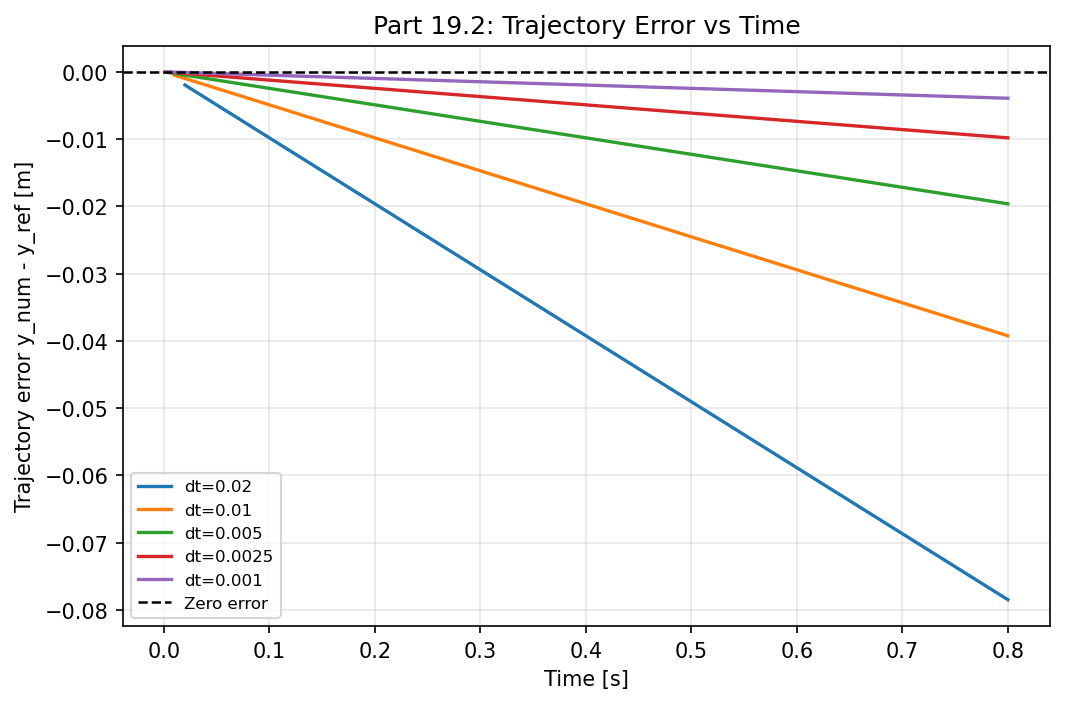
\includegraphics[width=\columnwidth]{part19_2_trajectory_error_overlay.png}
    \caption{Part 19.2: numerical trajectory error against analytical free-fall solution for multiple timesteps.}
    \label{fig:part19-trajectory}
\end{figure}

\begin{figure}[!t]
    \centering
    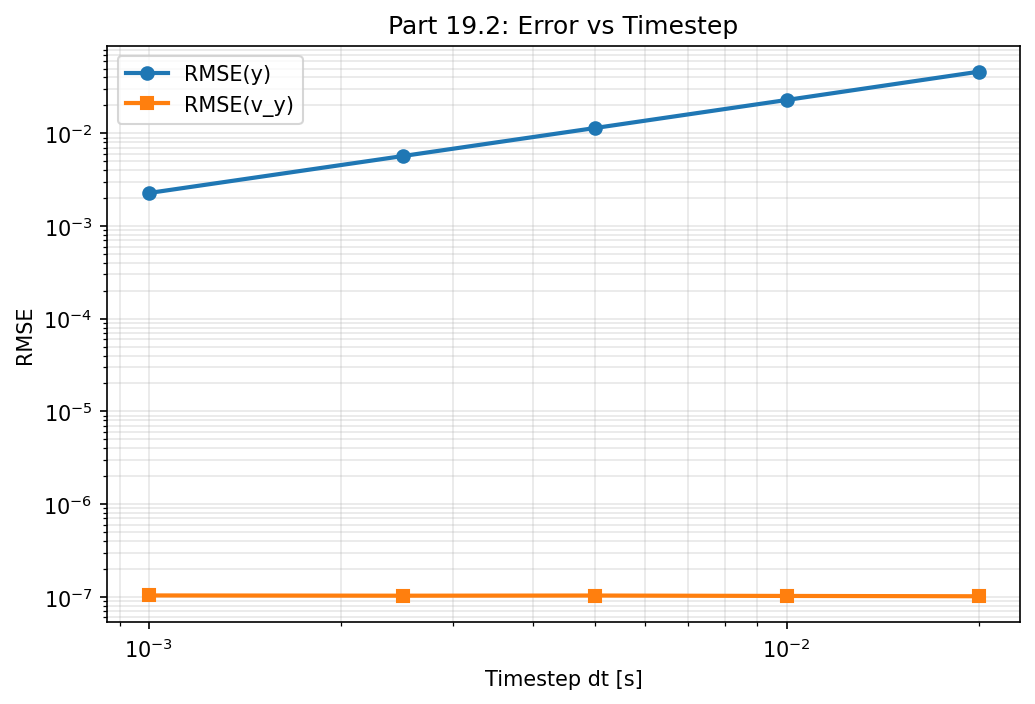
\includegraphics[width=\columnwidth]{part19_2_error_vs_dt.png}
    \caption{Part 19.2: error versus timestep.}
    \label{fig:part19-error-dt}
\end{figure}

\begin{figure}[!t]
    \centering
    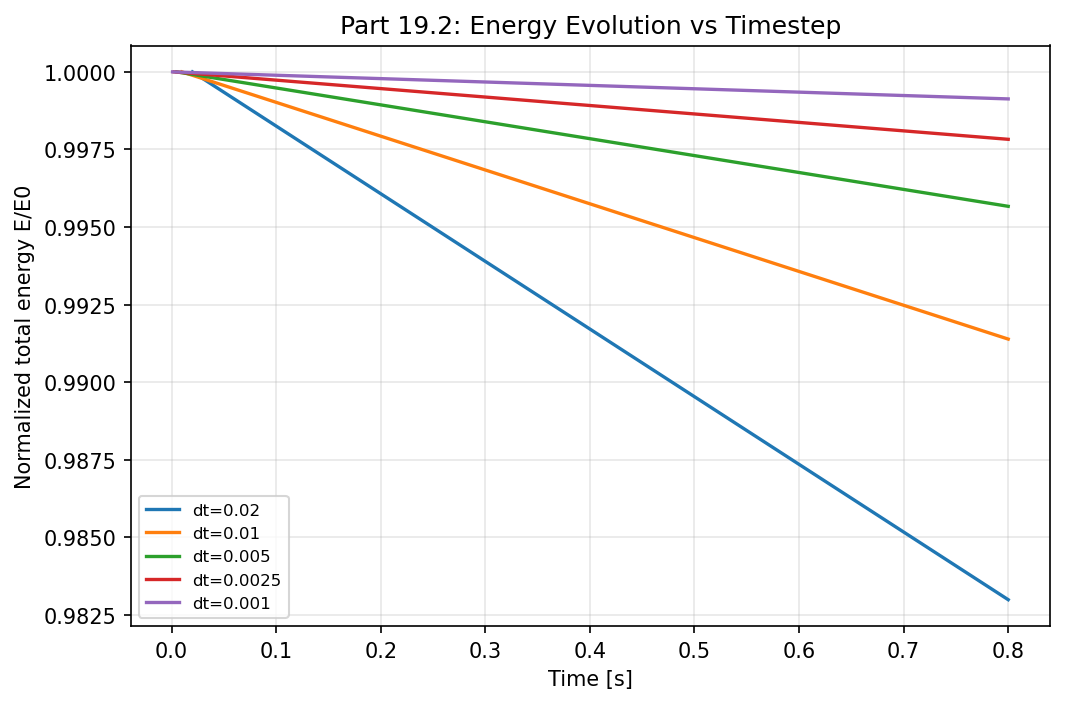
\includegraphics[width=\columnwidth]{part19_2_energy_evolution.png}
    \caption{Part 19.2: normalized total energy evolution for multiple timesteps.}
    \label{fig:part19-energy-evolution}
\end{figure}


\subsection{Automated Update Bundle}
The following subsections were generated directly from reproducible scripts and logs.

\subsection{Implementation and Validation Log (April 2026)}
The following updates were completed and logged for direct inclusion in the white paper.

\subsubsection{Bounce-Detection Robustness in Post-Processing}
The verification workflow was updated in \texttt{test\_verification.py} to avoid false bounce counts when output files were generated from a configuration different from \texttt{input\_config.in}. Two changes were applied:
\begin{enumerate}
    \item Physical time is now read from each VTK header (``Particle data at time ...'') rather than inferred only from a single external configuration file.
    \item Impact detection now uses a ground-contact-aware condition based on particle radius, combined with velocity sign-change and local-minimum filtering, followed by a small temporal de-duplication window.
\end{enumerate}
With these changes, the tuned bounce case reports five impacts in the $8\,\mathrm{s}$ analysis window at approximately $t=[0.96,\,2.79,\,4.54,\,6.22,\,7.82]$ s.

\subsubsection{Serial Profiling (Part 12)}
A dedicated profiling run was logged in \texttt{part12\_serial\_profile.csv} and \texttt{part12\_profile\_report.txt}. For case \texttt{part10\_n5000}, the measured serial runtime and distribution were:
\begin{itemize}
    \item total runtime: $2.0731\,\mathrm{s}$
    \item particle contact stage: $2.0384\,\mathrm{s}$ ($98.33\%$)
    \item output stage: $3.0803\times10^{-2}\,\mathrm{s}$ ($1.49\%$)
\end{itemize}
The dominant computational bottleneck is therefore the particle--particle contact stage.

\subsubsection{Parallel Correctness Checks (Part 13)}
Serial-vs-OpenMP comparisons were logged in \texttt{parallel\_validation\_report.csv} for $N=200,1000,5000$ and thread counts $p=2,4,8$. All checks returned \texttt{PASS} with
\begin{itemize}
    \item max absolute position difference: $0.0$
    \item max absolute velocity difference: $0.0$
    \item max absolute kinetic-energy difference: $0.0$
\end{itemize}
under the configured tolerances.

\subsubsection{Scaling and Amdahl Interpretation (Part 14)}
Performance artifacts were generated through \texttt{performance\_raw.csv}, \texttt{performance\_speedup.csv}, and \texttt{performance\_amdahl\_fit.csv}. Selected results at $p=8$ are:
\begin{itemize}
    \item $N=200$: $S(8)=0.969$, $E(8)=0.121$
    \item $N=1000$: $S(8)=1.722$, $E(8)=0.215$
    \item $N=5000$: $S(8)=2.248$, $E(8)=0.281$
\end{itemize}
This trend indicates that small systems are overhead-dominated, while larger systems amortize OpenMP overhead better. Fitted Amdahl serial fractions were approximately $f\approx0.49$ ($N=1000$) and $f\approx0.47$ ($N=5000$), consistent with non-ideal scaling.


\subsection{Bonus Part 18: Neighbour-Search Comparison}
A switchable contact-search implementation was added with \texttt{contact\_search\_method=0} (all-pairs) and \texttt{contact\_search\_method=1} (cell-linked).
Empirical candidate-pair scaling from the measured data is approximately $\mathcal{O}(N^{2.00})$ for all-pairs and $\mathcal{O}(N^{1.46})$ for the cell-linked strategy.
\begin{table}[!t]
\scriptsize
\centering
\caption{Part 18 neighbour-search comparison (serial runs)}
\label{tab:part18-neighbour-search}
\begin{tabular}{rcccccccc}
\toprule
$N$ & $t_{tot}^{AP}$ & $t_{tot}^{CL}$ & $S_{tot}$ & $t_c^{AP}$ & $t_c^{CL}$ & $S_c$ & Cand. factor \\
\midrule
200 & 0.0226 & 0.1932 & 0.12 & 0.0212 & 0.1914 & 0.11 & 80.57 \\
1000 & 0.5019 & 0.2230 & 2.25 & 0.4955 & 0.2164 & 2.29 & 102.69 \\
5000 & 12.5362 & 0.3839 & 32.66 & 12.5061 & 0.3554 & 35.18 & 458.85 \\
\bottomrule
\end{tabular}
\end{table}
where $t_{tot}^{AP}, t_{tot}^{CL}$ are total runtimes; $t_c^{AP}, t_c^{CL}$ are contact-stage runtimes; $S_{tot}, S_c$ are the corresponding cell-linked speedups over all-pairs; and Cand. factor is the candidate-pair ratio $N_{cand}^{AP}/N_{cand}^{CL}$.
Detected-contact counts match between methods for each tested $N$, confirming contact-search correctness while reducing candidate checks.
The measured candidate-pair reduction confirms why the baseline all-pairs method behaves as the expensive $\mathcal{O}(N^2)$ reference algorithm.
For small systems (here $N=200$), the cell-linked method is slower than all-pairs because grid build and traversal overheads dominate the reduced pair-check count.


\begin{figure}[!t]
    \centering
    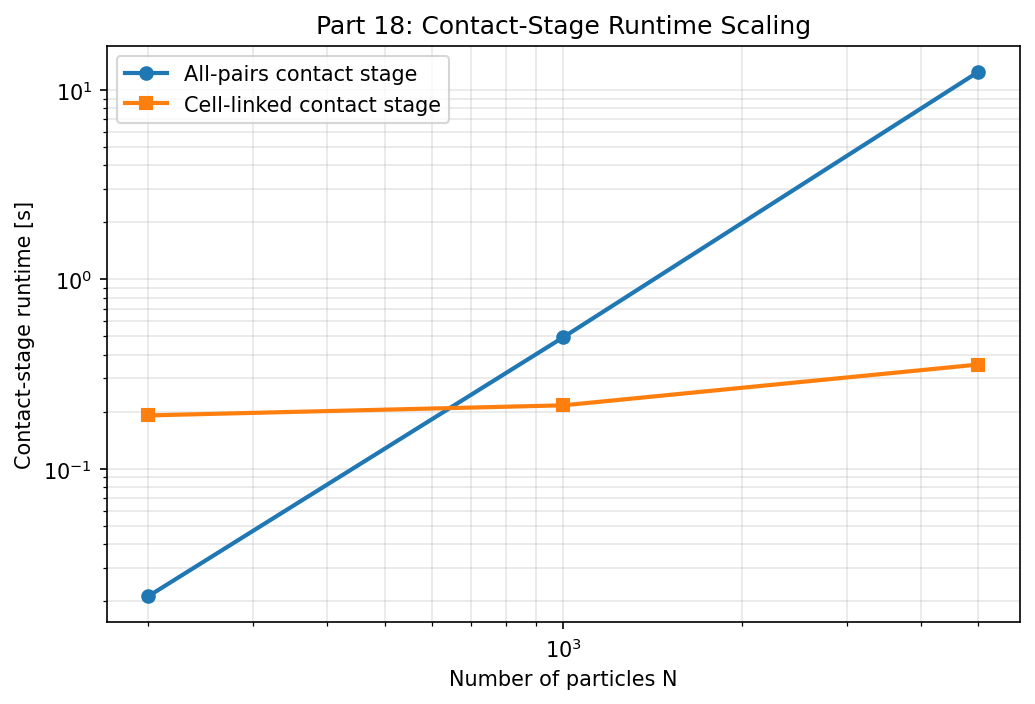
\includegraphics[width=\columnwidth]{part18_contact_runtime.png}
    \caption{Part 18: contact-stage runtime comparison between all-pairs and cell-linked methods.}
    \label{fig:part18-contact-runtime}
\end{figure}

\begin{figure}[!t]
    \centering
    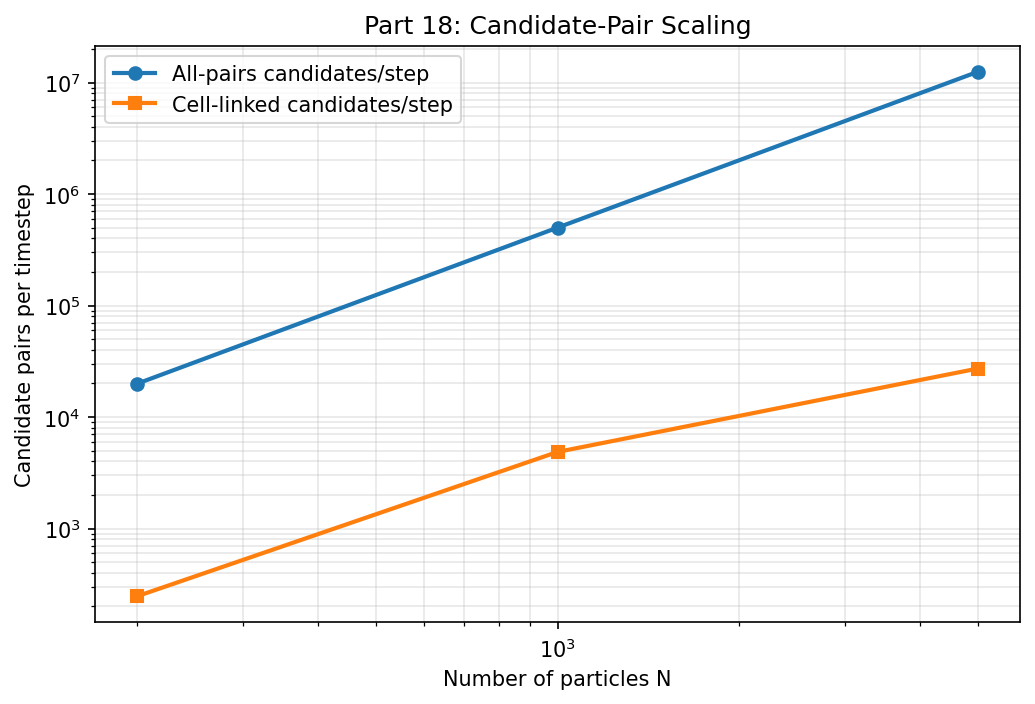
\includegraphics[width=\columnwidth]{part18_candidates.png}
    \caption{Part 18: candidate-pair scaling per timestep for all-pairs and cell-linked search.}
    \label{fig:part18-candidates}
\end{figure}

\subsection{Bonus Part 19.2: Timestep Sensitivity and Stability Limit}
A free-fall case without wall contact was simulated for multiple timesteps to quantify numerical accuracy and energy behavior.
\begin{table}[!t]
\centering
\caption{Part 19.2 timestep sensitivity metrics}
\label{tab:part19-2-timestep}
\begin{tabular}{rcccc}
\toprule
$\Delta t$ [s] & RMSE$(y)$ [m] & RMSE$(v_y)$ [m/s] & Max $|\Delta y|$ [m] & Max energy drift \\
\midrule
0.0200 & 4.616e-02 & 1.013e-07 & 7.848e-02 & 1.701e-02 \\
0.0100 & 2.287e-02 & 1.021e-07 & 3.924e-02 & 8.612e-03 \\
0.0050 & 1.138e-02 & 1.031e-07 & 1.962e-02 & 4.333e-03 \\
0.0025 & 5.677e-03 & 1.027e-07 & 9.810e-03 & 2.173e-03 \\
0.0010 & 2.268e-03 & 1.034e-07 & 3.924e-03 & 8.708e-04 \\
\bottomrule
\end{tabular}
\end{table}
A log-log fit gives an error slope of approximately 1.01 for position RMSE, which is consistent with first-order temporal behavior expected from semi-implicit Euler integration.
Velocity RMSE remains nearly timestep-independent at about 1e-7 m/s across all tested timesteps (slope -0.01), indicating that truncation error in this observable is already below a small floating-point and interpolation floor for this setup.
A Richardson three-grid analysis on final-height values gives observed orders between 1.00 and 1.00 (mean 1.00), consistent with first-order time integration.
\begin{table}[!t]
\centering
\caption{Part 19.2 Richardson observed order (final height)}
\label{tab:part19-2-richardson}
\begin{tabular}{rcc}
\toprule
$(\Delta t_c,\Delta t_m,\Delta t_f)$ [s] & $r$ & $p_{obs}$ \\
\midrule
(0.0200, 0.0100, 0.0050) & 2.0 & 1.00 \\
(0.0100, 0.0050, 0.0025) & 2.0 & 1.00 \\
\bottomrule
\end{tabular}
\end{table}
To connect this convergence study with stability limits, a bouncing test was run around a theoretical explicit-step threshold. Using a linear spring-mass estimate, the contact time is $t_c \approx \pi\sqrt{m/k_n}$ and the threshold used here is $\Delta t_{crit}=t_c/\pi$ \cite{edem_linear_spring,pfc_timestep}.
For $m=1.3$ kg and $k_n=1.0e+05$ N/m, this gives $t_c\approx 0.0113$ s and $\Delta t_{crit}\approx 0.0036$ s.
\begin{table}[!t]
\centering
\caption{Part 19.2 critical timestep check (bouncing case)}
\label{tab:part19-2-critical}
\begin{tabular}{rccc}
\toprule
$\Delta t$ [s] & $\Delta t/\Delta t_{crit}$ & Max $E/E0$ & Final $E/E0$ \\
\midrule
0.0030 & 0.83 & 1.39 & 0.83 \\
0.0040 & 1.11 & 9.40 & 5.26 \\
\bottomrule
\end{tabular}
\end{table}
The under-limit run ($\Delta t=0.003$ s) remains bounded but shows numerical energy gain (Max $E/E0=1.39$), whereas the over-limit run ($\Delta t=0.004$ s) exhibits rapid unphysical energy growth (Max $E/E0=9.40$), which is visible as a sharp upward trend in the critical-energy plot.


\begin{figure}[!t]
    \centering
    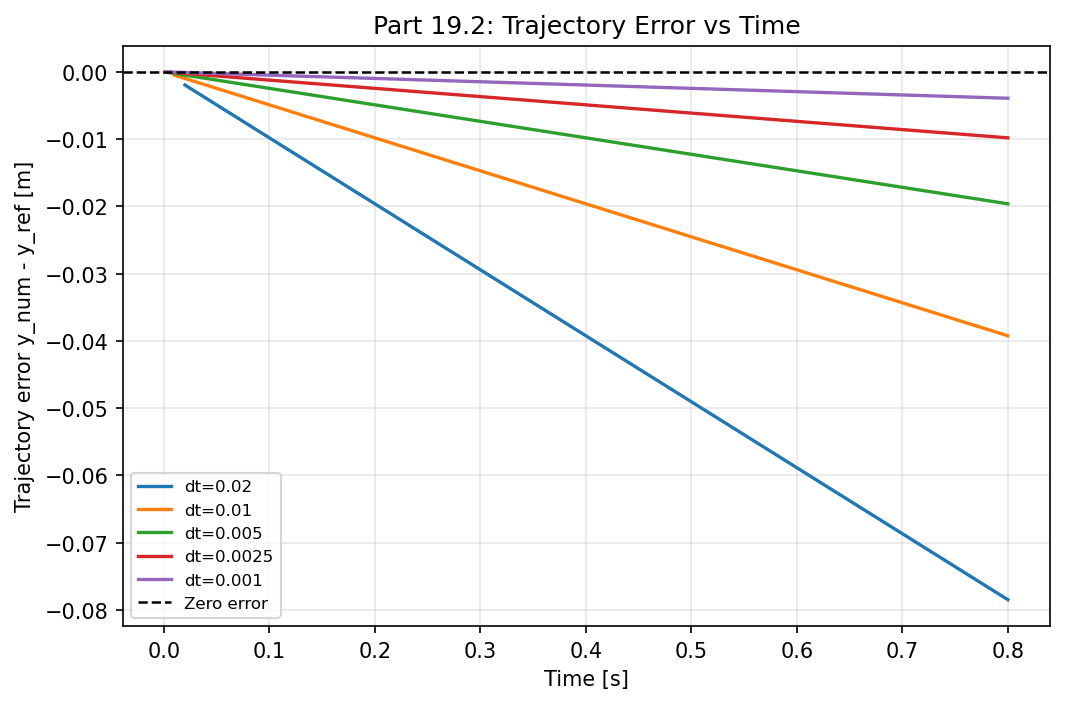
\includegraphics[width=\columnwidth]{part19_2_trajectory_error_overlay.png}
    \caption{Part 19.2: numerical trajectory error against analytical free-fall solution for multiple timesteps.}
    \label{fig:part19-trajectory}
\end{figure}

\begin{figure}[!t]
    \centering
    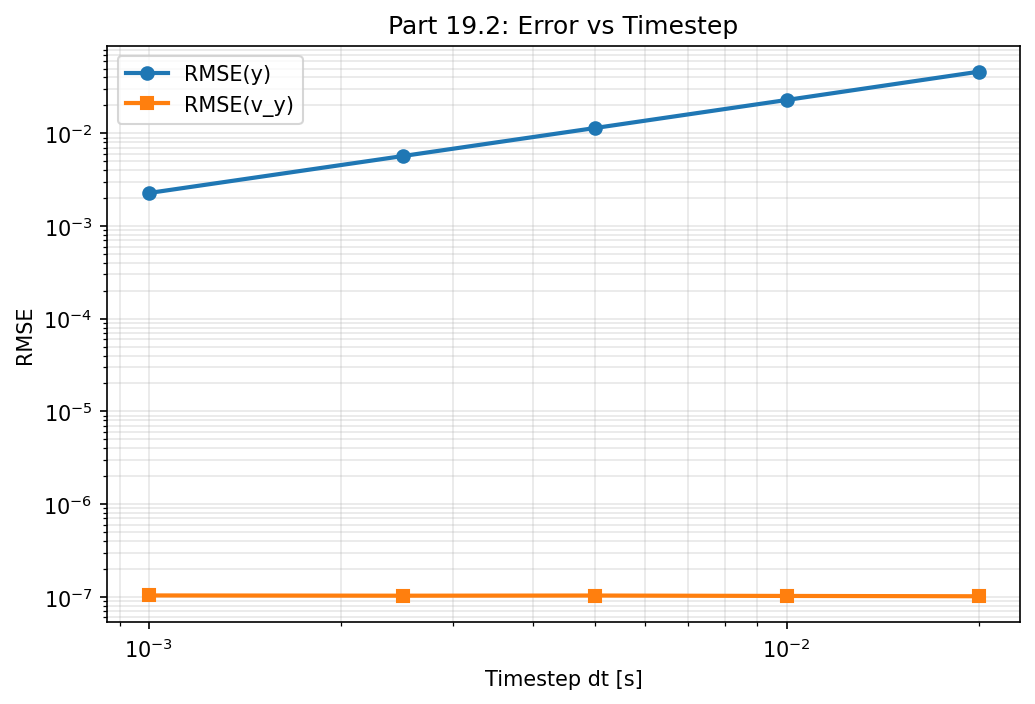
\includegraphics[width=\columnwidth]{part19_2_error_vs_dt.png}
    \caption{Part 19.2: error versus timestep.}
    \label{fig:part19-error-dt}
\end{figure}

\begin{figure}[!t]
    \centering
    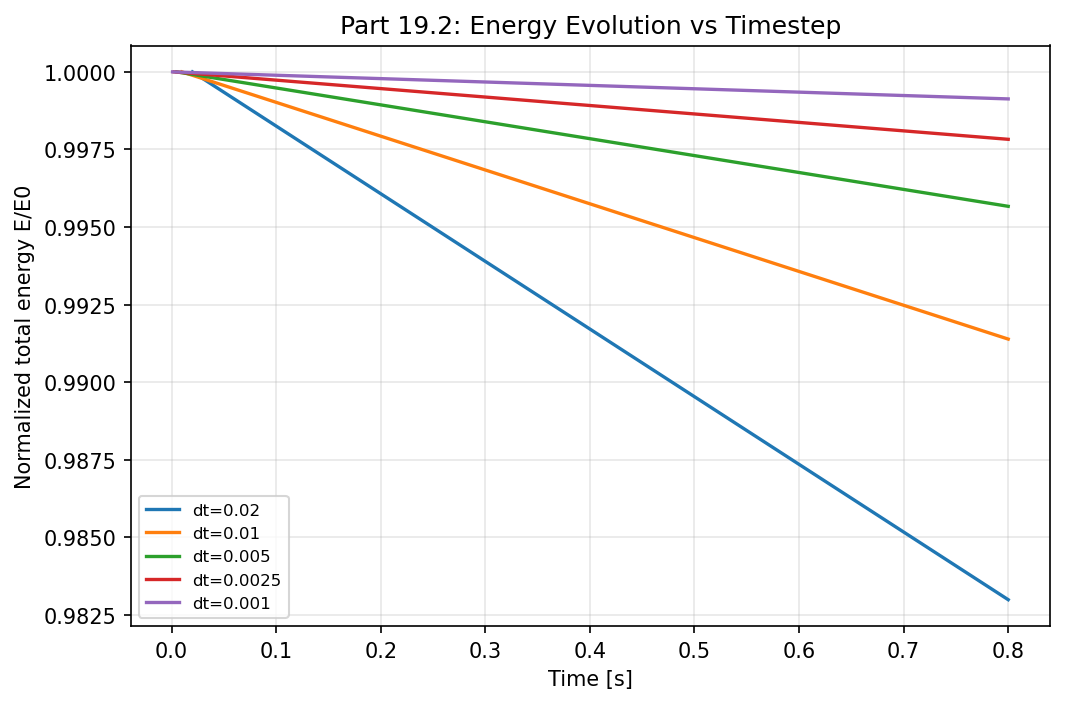
\includegraphics[width=\columnwidth]{part19_2_energy_evolution.png}
    \caption{Part 19.2: normalized total energy evolution for multiple timesteps.}
    \label{fig:part19-energy-evolution}
\end{figure}
